%%% ----------------------------------------------------------------
%% Thesis.tex -- MAIN FILE (the one that you compile with LaTeX)
%% ---------------------------------------------------------------- 

% Set up the document
\documentclass[a4paper, 11pt, oneside]{Thesis}  % Use the "Thesis" style, based on the ECS Thesis style by Steve Gunn
\graphicspath{Figures/}  % Location of the graphics files (set up for graphics to be in PDF format)

% Include any extra LaTeX packages required
\usepackage[square, numbers, comma, sort&compress]{natbib}  % Use the "Natbib" style for the references in the Bibliography
\usepackage{verbatim}  % Needed for the "comment" environment to make LaTeX comments
\usepackage{vector}  % Allows "\bvec{}" and "\buvec{}" for "blackboard" style bold vectors in maths
\hypersetup{urlcolor=blue, colorlinks=true}  % Colours hyperlinks in blue, but this can be distracting if there are many links.

%% ----------------------------------------------------------------
\newcommand{\vias}{$V_{bias}$}

%% ----------------------------------------------------------------
\begin{document}
\frontmatter      % Begin Roman style (i, ii, iii, iv...) page numbering

% Set up the Title Page
\title  {Thesis Title}
\authors  {\texorpdfstring
            {\href{your web site or email address}{Author Name}}
            {Author Name}
            }
\addresses  {\groupname\\\deptname\\\univname}  % Do not change this here, instead these must be set in the "Thesis.cls" file, please look through it instead
\date       {\today}
\subject    {}
\keywords   {}

\maketitle

\newcommand{\vias}{$V_{bias}$}
%% ----------------------------------------------------------------

\setstretch{1.3}  % It is better to have smaller font and larger line spacing than the other way round

% Define the page headers using the FancyHdr package and set up for one-sided printing
\fancyhead{}  % Clears all page headers and footers
\rhead{\thepage}  % Sets the right side header to show the page number
\lhead{}  % Clears the left side page header

\pagestyle{fancy}  % Finally, use the "fancy" page style to implement the FancyHdr headers

%% ----------------------------------------------------------------
%% Declaration Page required for the Thesis, your institution may give you a different text to place here
%\Declaration{
%
%\addtocontents{toc}{\vspace{1em}}  % Add a gap in the Contents, for aesthetics
%
%I, AUTHOR NAME, declare that this thesis titled, `THESIS TITLE' and the work presented in it are my own. I confirm that:
%
%\begin{itemize} 
%\item[\tiny{$\blacksquare$}] This work was done wholly or mainly while in candidature for a research degree at this University.
%
%\item[\tiny{$\blacksquare$}] Where any part of this thesis has previously been submitted for a degree or any other qualification at this University or any other institution, this has been clearly stated.
%
%\item[\tiny{$\blacksquare$}] Where I have consulted the published work of others, this is always clearly attributed.
%
%\item[\tiny{$\blacksquare$}] Where I have quoted from the work of others, the source is always given. With the exception of such quotations, this thesis is entirely my own work.
%
%\item[\tiny{$\blacksquare$}] I have acknowledged all main sources of help.
%
%\item[\tiny{$\blacksquare$}] Where the thesis is based on work done by myself jointly with others, I have made clear exactly what was done by others and what I have contributed myself.
%\\
%\end{itemize}
%
%
%Signed:\\
%\rule[1em]{25em}{0.5pt}  % This prints a line for the signature
%
%Date:\\
%\rule[1em]{25em}{0.5pt}  % This prints a line to write the date
%}
%\clearpage  % Declaration ended, now start a new page
%
%%% ----------------------------------------------------------------
%% The "Funny Quote Page"
%\pagestyle{empty}  % No headers or footers for the following pages
%
%\null\vfill
%% Now comes the "Funny Quote", written in italics
%\textit{``The roots of eduation are bitter but the fruit is sweet''}
%
%\begin{flushright}
%Aristotle
%\end{flushright}
%
%\vfill\vfill\vfill\vfill\vfill\vfill\null
%\clearpage  % Funny Quote page ended, start a new page
%%% ----------------------------------------------------------------
%
%% The Abstract Page
%\addtotoc{Abstract}  % Add the "Abstract" page entry to the Contents
%\abstract{
%\addtocontents{toc}{\vspace{1em}}  % Add a gap in the Contents, for aesthetics
%
%The Thesis Abstract is written here (and usually kept to just this page). The page is kept centered vertically so can expand into the blank space above the title too\ldots
%
%}
%
%\clearpage  % Abstract ended, start a new page
%% ----------------------------------------------------------------
%
%\setstretch{1.3}  % Reset the line-spacing to 1.3 for body text (if it has changed)
%
%% The Acknowledgements page, for thanking everyone
%\acknowledgements{
%\addtocontents{toc}{\vspace{1em}}  % Add a gap in the Contents, for aesthetics
%
%The acknowledgements and the people to thank go here, don't forget to include your project advisor\ldots
%
%}
%\clearpage  % End of the Acknowledgements
%%% ----------------------------------------------------------------
%
%\pagestyle{fancy}  %The page style headers have been "empty" all this time, now use the "fancy" headers as defined before to bring them back
%
%
%%% ----------------------------------------------------------------
%\lhead{\emph{Contents}}  % Set the left side page header to "Contents"
%\tableofcontents  % Write out the Table of Contents
%
%%% ----------------------------------------------------------------
%\lhead{\emph{List of Figures}}  % Set the left side page header to "List if Figures"
%\listoffigures  % Write out the List of Figures
%
%%% ----------------------------------------------------------------
%\lhead{\emph{List of Tables}}  % Set the left side page header to "List of Tables"
%\listoftables  % Write out the List of Tables
%
%%% ----------------------------------------------------------------
%\setstretch{1.5}  % Set the line spacing to 1.5, this makes the following tables easier to read
%\clearpage  % Start a new page
%\lhead{\emph{Abbreviations}}  % Set the left side page header to "Abbreviations"
%\listofsymbols{ll}  % Include a list of Abbreviations (a table of two columns)
%{
%% \textbf{Acronym} & \textbf{W}hat (it) \textbf{S}tands \textbf{F}or \\
%\textbf{LAH} & \textbf{L}ist \textbf{A}bbreviations \textbf{H}ere \\
%
%}
%
%%% ----------------------------------------------------------------
%%\clearpage  % Start a new page
%\lhead{\emph{Physical Constants}}  % Set the left side page header to "Physical Constants"
%\listofconstants{lrcl}  % Include a list of Physical Constants (a four column table)
%{
%% Constant Name & Symbol & = & Constant Value (with units) \\
%Speed of Light & $c$ & $=$ & $2.997\ 924\ 58\times10^{8}\ \mbox{ms}^{-\mbox{s}}$ (exact)\\
%
%}
%
%%% ----------------------------------------------------------------
%\clearpage  %Start a new page
%\lhead{\emph{Symbols}}  % Set the left side page header to "Symbols"
%\listofnomenclature{lll}  % Include a list of Symbols (a three column table)
%{
%% symbol & name & unit \\
%$a$ & distance & m \\
%$P$ & power & W (Js$^{-1}$) \\
%& & \\ % Gap to separate the Roman symbols from the Greek
%$\omega$ & angular frequency & rads$^{-1}$ \\
%}
%%% ----------------------------------------------------------------
%% End of the pre-able, contents and lists of things
%% Begin the Dedication page
%
%\setstretch{1.3}  % Return the line spacing back to 1.3
%
%\pagestyle{empty}  % Page style needs to be empty for this page
%\dedicatory{For/Dedicated to/To my\ldots}
%
%\addtocontents{toc}{\vspace{2em}}  % Add a gap in the Contents, for aesthetics


%% ----------------------------------------------------------------
\mainmatter	  % Begin normal, numeric (1,2,3...) page numbering
\pagestyle{fancy}  % Return the page headers back to the "fancy" style

% Include the chapters of the thesis, as separate files
% Just uncomment the lines as you write the chapters

\chapter{Introduction}

There are many kinds of particle detectors ranging from the first Bubble and Cloud Chambers up to the latest High Voltage CMOS (Complementary Metal Oxide) solid state detectors. Their detector design varies depending on many parameters: application, magnetic field, operational temperature, active medium, measurement rate, layout, radiation damage they can withstand... making it possible to optimise detectors for specific needs. During the past decades, silicon has become the technology of choice for tracking detectors, as it tends to offer an excellent compromise between energy, space and time resolution at a fairly moderate price. Another advantage of silicon detectors is the existing R\&D for other applications, and the possibility to go on commercial technologies.

 The scope of this work is the modelling of the performance of silicon detectors exposed to high fluence of particles, such as those existing in particle accelerators, like the Large Hadron Collider (LHC) at CERN\footnote{Conseil Européen pour la Recherche Nucléaire}. There, the innermost tracking detectors will have to withstand particle fluences up to $10^{16}$ $n_{eq}/cm^{2}$  during 10 years of operational lifetime. The amount of collected charge will decrease over this period due to trapping of charge carriers in radiation induced traps. The detectors will have to be designed such that the charge loss is above an electronics threshold of $\approx$ 6000 $e^{-}$, which is the minimum the electronics can resolve. 

 Understanding the effects of radiation in Si is a crucial task. These detectors have to operate for a period of 10 years without being replaced. In this project, a model of radiation damage in silicon has been implemented into an already existent simulation software called TRACS\cite{TRACS}. 
 
In Chapters \ref{chap:detector} and \ref{chap:rad} we will introduce some background information on how silicon detectors work and how radiation affects silicon internal structure and performance. Chapter \ref{chap:TCT} will describe an experimental technique used in this work to characterise silicon detectors. This data will serve as an input to crosscheck the results of the simulation. In chapter \ref{chap:tracs} the inner workings of the software and the actual implementation of radiation damage is presented. At last, chapter \ref{chap:TRACSvalidity} will show a comparison between simulation and experimental data to prove the validity of the simulations. 

%\section{Solid State Detectors in High Energy Physics}
%
%In this section we shall clarify how and why particles are detected using solid state detectors in particular Si. 
%
%\subsection{Principles of particle detection}
%
%It should be clear how particles are detected in almost every single detector existing today: Have detector with Electric field inside; particle goes boom; boom creates charges; charges drift in electric field; drift generates signal; signal tells how is the particle that went boom. This could be a good place to introduce concepts such as 
%
%\subsection{Specific charateristics of a \textit{Si}-based particle detector}
%
%In this subsection we should tackle everything specific to \textit{Si} detectors, from te advantages over gas detectors to the technical details of their design and operation. Typical numbers can be helpful. The Diode should be explained in detail and its importance in research and understanding should be clear in a context where nobody actually detects particles with them anymore. Should we explain detailed the semiconductors and p-n junction?
%
%\section{Radiation damage in \textit{Si} detectors}
%
%We should clearly explain the effects of radiation in \textit{Si} without going too deep in the differences between proton-like and neutron-like. We can only afford to go deep into traps and trapping as well as space charge modification inside the detector. Leakage current, higher vdep, etc. should be mentioned as wel.
3 % Introduction

\chapter{Silicon detectors: all you always wanted to know but never dared asking} %PREELIMINARY TITLE % (fold)
\label{cha:simulator_development}

Silicon detectors work using the same basic principles that almost every other particle detector uses. This classical "detector configuration" consists fundamentally in an enclosed volume which is filled with a material in which free charges can be generated by and incident particle. This volume is then connected to an electrical circuit that creates a  potential difference between two points inside the volume, these can also be part of the edge of said volume. The process by which signal is collected is very easy to understand in this general detector.

When an incoming particle goes through the volume there's a probability that this particle might create one or more pairs of free charges, one positive and one negative (either electron-ion or electron-hole pair), these charges then move in the electric field inside the volume following opposite trajectories depending on their charge. The movement of charges creates a current in the circuit by electrical induction that depends on the speed of the charged particles and the total amount of charge. This current created in the circuit is what can be measured in the lab and analysed to obtain all the relevant physical quantities.

Even though this general concept of particle detector holds true for almost every detector in use nowadays the implementation of this concept varies greatly depending on the material from which the detector is constructed. In the following sections we will see in detail how silicon can be turned into a particle detector as well as the operational principles of silicon detectors

\section{P-N Junction}

Silicon is a semiconductor material and as such it has some interesting properties. In a pure state silicon does not conduct electricity well enough to make for a good detector material. However, as any semiconductor its electrical properties can be easily modified by adding controlled impurities a pure silicon crystal; this process is called doping. There are two main types of impurities used for silicon doping: acceptor impurities and donor impurities.

Donor impurities have one electron more in the outer shell than silicon. Donor impurities introduce extra energy levels close to the Conduction band filled with the extra electrons they bring. Conversely acceptor impurities have one less electron in the outer shell producing new empty energy levels close to the Valence band. These last empty energy levels are better pictured in solid state physics as being filled with a hole\footnote{Holes are quasi-particles used in solid state physics as a more convenient way of describing the lack of an electron} since it groups all the effects of the electrons moving in and out of empty energy levels into one particle.

These donor (or acceptor) levels introduced by impurities are very close to the conduction (Valence) band, so much so that energies of the order of $k_B T$ at room temperature are enough to excite electrons into the conduction band (from the valence band into the impurity level). These excitations result in the doped silicon being able to conduct electricity much better than before and allowing silicon to be used as detector material.

Silicon can be doped with donor impurities only, acceptor impurities only or both types of impurities. In the latter case is the difference between the number of donor impurities ($N_D$) and acceptor impurities ($N_A$) dictates whether the doped silicon will be considered $p$-doped ($N_A > N_D $) or n-doped ($N_D > N_A$). When $n$-doped and $p$-doped silicon are put in contact or when there is an abrupt jump in the silicon from $n$-doping to $p$-doping, the so called $p-n \hspace{5pt} junction$ appears and some strange effects appear.

To understand what are those effects and why they happen we should start by looking at each type of silicon on both sides of the junction. On the one hand we have and excess of acceptors $N_A$ ($p$ side) whilst on the other side there is an excess of donors $N_D$ ($n$ side) this produces a gradient of the chemical potential that makes impurities diffuse from one side to the other. This diffusive migration of donor impurities to the $p$ side and acceptors to the $n$ side creates an electrical potential difference due to said movement of charged impurities from one side to the other. The resulting electric field produces the opposite effect in the charged impurities than the chemical potential. Since the ionised atoms in the silicon lattice cannot effectively move from their initial positions, an equilibrium is achieved when the chemical and electrical potentials balance its effect resulting in an steady state. 

In such a equilibrium state 2 zones can be clearly identified near the $p-n$ junctions, on top of the unaffected $p$ and $n$ regions of the silicon far away from the junction. These two zones are electrically charged having an excess of negative charge on the $p$ side and a excess of positive charge on the $n$ side of the junction. In this region, called the space charge region, an electrical field and its correspondent potential can be found. This region is called the depletion region because it has been depleted of free charge carriers.

\subsection{Effective space charge distribution ($N_{eff}$)} 
%Talk equations and introduce the concept of Neff and its shape in a non-irradiated silicon detector

The electrical properties of the $p-n$ junction can be derived from the corresponding Poisson equation. 
\begin{equation}
\nabla^2 \phi = \frac{\rho(x)}{\epsilon} 
\label{eq:poisson}
\end{equation}

Where $\phi$ is the electric potential, $\epsilon$ the absolute permittivity of silicon and $\rho(x)$ is the space charge distribution as a function of position.

It is easy to see from equation (\ref{eq:poisson}) the important role of the space charge distribution, also called $N_{eff}$. Such quantity will also play a very important in the parametrisation and implementation of radiation damage in the TRACS simulator, as we will explain in detail in sections [SECTION]. For now, we will focus on the non-irradiated case in which the $N_{eff}$ is constant throughout the depleted zone \[ Kramberger (2.5)\] for a junction located at $x=0$ and $-x_p$ and $x_n$ being the extremes of the depleted zone.

It is important to note that since the both the $n$-doped and $p$-doped silicon were electrically neutral in the beginning and no charge has been created or destroyed in the process of creating the junction, the material as a whole must also be neutral which means the total amount of charge has to be equal on both side, this leads us to a very important conclusion when building a detector out of silicon: \[N_A x_p = N_D x_n\] 

This relationship is very important when building a detector since one tries to maximise the sensing volume of the detector (which in a silicon detector is the depleted zone) but the $p-n$ junction is a feature to avoid in the middle of the detector. The usual procedure when building a silicon detector is to have one of the doped silicon sides be of a much higher doping than the other (e.g.: $N_A >> N_D$  so that the depletion zone is almost entirely on one side of the junction ($x_n >> x_p$). In this manner one gets rid of the mess involved in having the $p-n$ junction in the middle of the detector.

With this configuration one can make useful approximations to calculate the width of the depleted zone ($w$) such as $w \approx x_p$  (using the example above) so that $w$ can be calculated using 
\begin{equation}
w = \sqrt{\frac{2\epsilon V_0}{\epsilon_0 N_D}}
\label{eq:width}
\end{equation}

where $V_0$ is the so called built-in potential difference mentioned before that arises from the diffusion of the impurities from one side to the other of the junction.

When Poisson's equation is solved for $\rho = const$ the resulting electric $\nabla \phi = \vec{E}$ field is linear with the distance to the $p-n$ junction. In a typical detector configuration (where $w \approx x_{p/n}$) this mean there is an electric field across the whole active volume of the detector (depleted area) in which any carrier created inside of the depleted zone will drift out of said zone. This configuration is exactly what we described at the begging of the section as the basic "detector configuration". 

The presence of the $p-n$ junction is, therefore, the fundamental way to make a particle detector out of silicon and its properties will determine the effectiveness of said detector. However, this basic configuration is usually not enough to have a silicon detector that can be use in real-world applications. To get a "usable" silicon detector one should build upon the features we have seen to enhance its properties as we will see in the next section.

\section{Detector configuration and signal creation}

The first problem that one faces when building a silicon detector from a bare $p-n$ junction is getting as much active volume as possible i.e.: depleting the whole piece of silicon. For this purpose a bias voltage ($V_{bias}$) is introduced. This $V_{bias}$ is applied externally following the same polarity as the built-in potential $V_0$ and increases the depleting effect of the $p-n$ junction therefore increasing the active volume of silicon. 
To calculate the effects of the \vias it is enough to substitute $V_$ by the sum of both potentials ($V_0$ +\vias) in equation (\ref{eq:width}). The resulting equation can be simplified if we assume $V_0 << $\vias which holds true in most of the real-world cases. This means equation (\ref{eq:width}) can be re-written as: 
\begin{equation}
w = \sqrt{\frac{2\epsilon V_0}{\epsilon_0 N_D}}
\label{eq:widthVias}
\end{equation}

What this equation shows is that the depleted silicon volume can be as big as desired, provided that enough voltage is applied, making it possible for the whole silicon volume to be depleted and used as a particle detector. 

These basic principles allows silicon detectors to be made but since there are very small geometrical restrictions to create a $p-n$ junction, silicon detectors come in ever so increasingly more complex configurations. From the very new LGADs (with built-in gain) to the widespread micro-strips (used in most of the inner parts of the experiments at LHC) the design, properties and fabrication processes vary extremely. However the silicon pad detector remains one of the most important detector designs, particularly in research, due to its simplicity. This simple detector configuration allows researches to understand the fundamentals of silicon detectors without any design feature getting in the way. 

A silicon pad detector has the most simple structure possible and its composed of a thin (typically ~3$\mu$m) layer of very highly doped silicon called the implant that sits on top of a bigger (typically 300$\mu$m) piece of silicon with a lower density of dopants called the bulk. These two piece of silicon have different type of dopants to create the $p-n$ junction. Connection to the electrical circuit that provides the \vias and performs read-out of the signal is done by means of an ohmic metal contact in the top part of the pad (on top of the thin layer).On the other side of the bulk there's another highly doped layer of silicon and another metal ohmic contact is placed on top of it for better electrical contact with the circuit.

\section{Signal Generation: Ramo's Theorem} % No es Sergio Ramos, es otro Ramo's

The depleted part of the silicon detector, i.e.: the active part is the volume of silicon in which free charge carriers might be created and then drift creating an electrical signal that can be measured and analysed in the laboratory. When an incoming particle goes through thew bulk of the silicon detector it can create electron-hole pairs. The number of pairs created will depend on the particle's nature and energy and has an obvious and direct impact in the collected signal. 

When a particle is able to knock off one electron out of their original position, it will move to an energy level in the conduction band, leaving a hole in the valence band. This yields a situation in which both the electron in the conduction band and the hole in the valence band can move in the electric field present inside the depleted bulk of the detector. This drift of the charge carriers inside of the depleted region will induce a signal in the electrodes of the circuit as explained by Ramo-Shockley Theorem.

The Ramo-Shockely Theorem states that the current induced by a moving charge on a wire/circuit is proportional to the carge of the particle and the velocity at which it moves. 
\begin{equation}
	i = v \cdot q
	\label{eq:ramo} 
\end{equation} 
For a system where more than one particle is moving and thus inducing current in the circuit, the total current can be written as the sum of each individual contribution from the N particles moving in the system. If all the charge carriers have the same charge as it is in the case of electrons and holes drifting inside the silicon volume, then equation (\ref{eq:ramo}) can be re-written as:
\begin{equation}
	I = q \cdot \sum_{n=1}^{N} v_n 	\label{eq:ramoTot} 
\end{equation} 

In semiconductors like silicon the drift velocity of electrons and holes can be parametrised as the product of the electric field ($ \vec E $) and the mobility (\mu) of said particle.\[v = \mu \cdot \vec E\] Where the mobility is and experimentally determined parameter that parametrises how a charge carrier moves in a given energy band when subject to an electric field. Typically electron mobilities ($ \mu_e $) are taken to be referred to the conduction band unless otherwise specified. Conversely, hole mobilities ($ \mu_h $) are taken to be referred to the valence band by default. Putting all this together we arrive at
\begin{equation}
	I = q \cdot \sum_{n=1}^{N} \mu_i \cdot \vec{E} 
\label{eq:ramoMob}
\end{equation}
where the sub-index $i$ may refer to electrons or holes depending on the particle that contributes to the total current.

This theorem and its results are one of the most fundamental principles needed to understand silicon detectors. In fact, its applicability goes beyond silicon unirradiated silicon detectors and holds true for irradiated silicon detectors. It is important to note, though, that for irradiated silicon detectors there are some factors to take into account that makes the application of Schockley-Ramos theorem less straight forward than in the unirradiated case. In the following section we will go in more detail about what are the effects of irradiation in signal formation and collection as well as explain how to properly take into account those effects.
 % Simulator Development and results 

\chapter{The effects of radiation in silicon detectors}% No definitivo
\label{sec:rad}
% I haven't talked about leakage current and I most certainly should

When a particle goes through a silicon detector, it can loose energy via ionization, which is a reversible process because the electrons extracted from the atoms will end up recombining. The particle can also lose energy via non-ionizing interactions, where the particle interacts with the Silicon atoms or with the dopant atoms. The effect is detrimental for the detector and leads to a reduction of the collected charge, amongst other macroscopical effects. It is important to understand these changes and have a parametrisation of the degradation. Understanding these defects is fundamental for designing radiation-hard detectors.

In this chapter we summarise the most important mechanisms of radiation damage. One of the key points of the project was to implement radiation damage on the TRACS simulator.


\section{Damaging the lattice}% No definitivo

\begin{figure}[H]
	\centering
	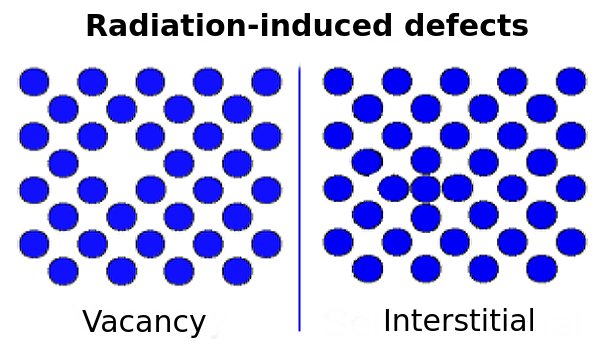
\includegraphics[width=0.8\textwidth]{chap3_defects.png}
	\caption{Interstitial (right) and Vacancy (left) lattice defects are illustrated here. This defects are be created inside silicon detectors after irradiation.}
	\label{fig:IV}
\end{figure}

When a particle transversing the silicon detector undergoes a non-ionising interaction one or more atoms get knocked-out from their equilibrium position in the lattice, disrupting the ordered structure of silicon. If the atom does not return to the equilibrium position, and Interstitial-Vacancy (I-V) defect is created. The term Interstitial refers to the knocked-off atom missplaced in the lattice and the Vacancy refers to the empty place that it leaves behind as shown in Figure \ref{fig:IV}. This type of defect alters the ordered structure of the lattice and creates new energy. The mechanisms by which the I-V defects degrade the performance of the detector and its practical consequences will be discussed in the next sections.

%When a particle goes through a silicon detector it can ionise the material and move electrons out of the valence band into the conduction band generating an electrical signal than be read, as we have previously discussed. Another possibility is that the particle knocks off one or more of the silicon atoms that compose the lattice. In this case the atom might return to its original position if the momentum transfer is small dissipating the extra energy via thermal vibrations or it might get knock off completely from its original position. In the latter case the lattice presents now a defect that will influence its properties. For this section we will only focus on the types of defects and their evolution, leaving their effects to the next two sections. 

An inpinning particle can create more than one I-V defects provided it has enough energy. The second I-V defects can be created directly by the particle or by the recoil atom if enough energy was transferred to it. The size and clustering of the defects depends on the energy and type of radiation. 

%During the radiation process, either in a controlled environment for research purposes or as a side effect of particle detection, various types of particles with different energies might transverse the silicon detector might have different damaging effects in the silicon lattice. When an inpinning particle knock off an atom the result is an interstitial-vacancy pair. The knocked-off atoms sitting in a different position between other silicon atoms is what we call interstitial defect and the lack of such atom on its original position is called vacancy. Depending on the inpinning particle type and the energy transferred to the recoil atom more than vacancy-interstitial defects might be created after the first impact. The size and clustering of these defects depends strongly on the energy of the particles and also on their characteristics. 

For example, according to \cite{MMoll}, photons with up to 1 MeV energies will create only point defects with no clustering effects. Electrons can create both point defects and clusters of defects, with clusters only occurring for electron energies above 8 MeV. Neutrons will create mainly clusters starting at energies as low as 35keV. 

Typically the NIEL (Non-Ionising Energy Loss) hypothesis is used to characterise the radiation damage caused by any type of particle. The NIEL hypothesis states that the damage produced by radiation of any kind of particle is proportional to the damage produced by 1 MeV neutrons. Therefore fluence of any type of radiation is rescaled to the equivalent fluence of 1MeV neutrons. %the standard unit of measuring the radiation that a silicon detector has undergone is the neutron equivalent (neq).

The I-V defects induced by radiation are not necessarily static defects and their size and configuration may vary in time. The damage due to radiation evolves with time. For instance, the depletion voltage first decreases with time at a fixed temperature (so-called beneficial annealing) to increase linearly afterwards (long term annealing). The evolution speed depends heavily on temperature. Evolution achieved in around 21h at 60C can be slowed down to about 500 years just by cooling down the irradiated detector to -10C. 

The standard procedure followed by researchers includes an intentional annealing phase so that all irradiated detectors have undergone similar damage evolution. The annealing time depends on the transport and irradiation conditions. Irradiated sensors are stored in cold environments such as fridges.

%Another important aspect of radiation damage and radiation-induced defects is their evolution in time. It has been shown that the effects of radiation on silicon detector evolve with time even after the irradiation has been stopped. Studies on annealing of irradiated silicon detectors show that typically there is a beneficial evolution right after the irradiation process in which the silicon damage becomes smaller. After this stage annealing increases the damage on irradiated silicon detectors with time reaching levels well over the initial state right after irradiation. This process can be slowed down by lowering the temperature of the detector. Evolution achieved in around 21h at 60C can be slowed down to about 500 years just by cooling down the irradiated detector to -10C. It is for this reason that silicon detectors are usually annealed for a short period of time after irradiation, and the stored at low temperatures for transport and experimental measurements.

\section{Trapping effects} % No definitivo
\label{sec:trapEfect}

%Defects in the silicon lattice have no effect in the generation of $e-h$ pairs but do have an effect in their drift and collection. This is due to the defects introducing what are called $deep$ levels. Such deep levels lie in the gap between the conduction and valence bands but much further from them than the shallow levels introduced by impurities as explained in section [SECTION].

%Deep levels can be filled by electrons or holes depending on their proximity to the valence or conduction band respectively. The main effect of these deep levels is trapping charge carriers for a large amount of time compared with typical collection times in non-irradiated silicon detectors. The trapping of the charge carriers modifies that distribution of electrons and holes inside the detector which in turn can significantly modify the space charge distribution inside the depleted region of the detector. The drift of both charge carriers is also affected by these changes as we will see in detail later. In special cases the effect can be so strong that type inversion might occur. When this happens the previously $p$ doped part of the silicon detector becomes effectively $n$ doped. This effect of type inversion does not happen in initially $n$ doped silicon.

%If one looks at the radiation-generated deep levels, they can hold charge carriers for long times before realising it. This process disrupts temporarily the $N_{eff}$ inside the silicon detector. If the trapping-releasing cycle happens with enough frequency (as it is the case under most circumstances) then the \neff can be thought of being permanently modified by the charges trapped in the deep levels. As opposed to the unirradiated case, now the \neff is not a constant but has a different shape. Since the \neff is one of the most important things in signal development inside the silicon detector, it is of great importance that its modification due to radiation damage are well known.

%Being, as it still is, a body of great debate, \neff parametrisation has yet to find a definitive answer that can be successfully applied in all cases. For now we will focus on mainly two parametrisation of said variable for those two are the most succesful and widely accepted, but it should be noted, again, that \neff evolution with radiation damage is not fully understood at the time of writing this work. First of the parametrisation was introduced in 2002 and devised the \neff inside the detector to change shape from constant to linear with depth. In this model the already present electric field inside the detector would force influence charge carriers to move to both ends of the detector (depending on the charge sign) creating an excess of positive charges on one side and a excess of negative ones on the other compared to the non-irradiated state. The resulting \neff is a straight line that gives rise to a parabolic electric field that will change the shape of the collected signal in accordance to experimental results.

%The second mayor parametrisation that should also be considered in the frame of this project is a variation on the basic fundamentals of the linear model. This next model was proposed more recently by G.Kramberger and states that the shape of \neff after irradiation can be parametrised in some cases as being constant in three separated regions. As it can be seen in Figure FIGURE\_3ZONE\_NEFF each of the three parts of the \neff would be constant generating a linear electric field with three different slopes resembling the shape of the aforementioned parabola that is observed experimentally.

The defects induced by radiation only affect the drift and collection of the $e-h$ pairs. The I-V defects create the so called $deep-levels$ that can trap and hold charge carriers for times longer than the typical collection times in silicon detectors. The result is a net loss in charge collection efficiency as well as a modified \neff profile.

\begin{figure}[H]
	\centering
	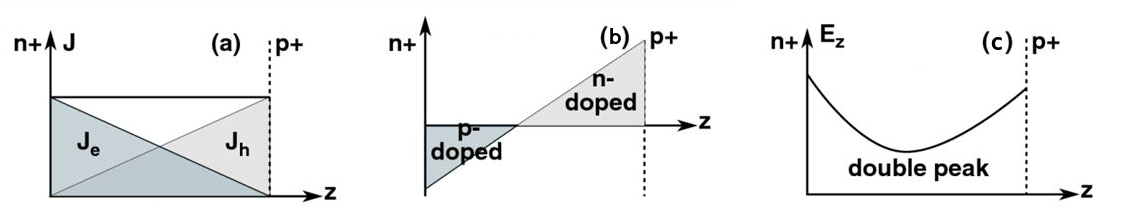
\includegraphics[width=0.8\textwidth]{chap3_erem.jpg}
	\caption{Interstitial (right) and Vacancy (left) lattice defects are illustrated here. This defects are be created inside silicon detectors after they have been irradiated.}
	\label{fig:Eremin}
\end{figure}

To explain why the \neff gets modified after irradiation, we will follow the argument presented by V.Eremin\cite{Eremin}. The current density of $e$ or $h$ ($j_i(z)$), in a fully depleted silicon detector, is not a constant but has a linear dependence with thickness ($z$), as shown  in figure \ref{fig:Eremin}\emph{a}. The concentration of carriers ($n_i(z)$) is proportional to the current $j_i(z)$, so $n_i(z)$ is also linear with $z$. After enough radiation the defects and their correspondent deep levels can be considered uniformly distributed throughout the detector. The amount of carriers trapped can be considered proportional to their concentration. Taking the charge sign into account the end result is a linear dependence of space charge distribution with $z$ (Figure \ref{fig:Eremin}\emph{b}. For a more complete description of this argumentation and its validity the reader is referred to the bibliography.


% Consecuences of a modified Neff (leakage current, higher Vdep, type inversion, DP & DJ)

One of the consequences of having a non-constant \neff configuration is that the resulting electric field inside the detector gets modified. In the linear case mentioned above a parabolic electric field appears (see Figure \ref{fig:Eremin}\emph{c}) giving rise to a characteristic \emph{double peak} (DP) shape of the transient waveforms. Another consequence of not having a constant \neff is the appearance of a second $p-n$ junction at the end of the detector creating the double junction (DJ) effect. The apparition of the DJ means that in a detector not fully depleted both ends remain sensitive to radiation.

%Other effects of the modified \neff of lesser importance for this project are the increase in leakage current, a higher \vias needed for depleting the full detector volumen, and more exotic processes such as type inversion. % Deberia hablar algo mas de type inversion? decir lo que es?

% EXPLAIN WHY IT MIGHT NOT BE LINEAR but something more exotic (link with TRACS capabilities)

So far it has only been considered that the modification of the \neff due to radiation-induced defects gives rise to a linear \neff inside the detector. However, this might not be always the case, as it has been proposed in more recent publications\cite{KramVertex}. Analysis performed using edge-TCT techniques suggest that the \neff configuration might have three different regions in which its value remains constant. This parametrization will be referred to as \emph{triconstant} and can also explain the DJ and DP effects seen experimentally. As it will be explained in detail later, both linear and triconstant parametrisations have been implemented into TRACS as well as a third parametrisation consisting of three linear regions.  

On top of the \neff modification, the deep levels induced by radiation have also an impact on signal collected from the detector. When charge carriers drift through the irradiated volume they may get trapped in a radiation-induced defect and remain there for as long as several miliseconds. This is much longer than the collection time (of the order of tens of nanoseconds) so they are effectively lost. As a result, the waveform shape gets distorded (as it will be explained in the following section) and the charge collected decreases worsening the performance of the detector.

\section{Signal degradation} % No definitivo
\label{sec:signalDeg}

%After taking a look at the effects that radiation has on silicon it is important to understand how radiations changes the read-out signal, since that is what will be measured in the laboratory. As we have already mentioned the main effect of radiation damage from a practical point of view is the creation of deep levels inside the band gap that act as trapping centers for the charge carriers moving inside the silicon bulk. For the sake of simplicity and ease of explanation when explanation when talking about the implementation of radiation damage in the software TRACS, we will treat \neff deformation as a different effect. This is very practical as it helps understand dynamical and static effects separately. 

%The effect that deep levels have in the signal is the trapping of the charge carriers creating a loss in charge collection efficiency. Because collection times in silicon detectors are of the order of tens of nanoseconds whilst the trapping times are typically of the order of milliseconds, the trapped carriers will never be released in time to be collected and are effectively lost. The process of trapping is a statistical one with the probability of one charge carrier to be trapped after a drifting inside the silicon for a time $t$ being  \[FORMULA FOR TRAPPING PROBS\] where $\tau$ (trapping time) is an experimentally determined parameter that shows how likely it is for a carrier to get trapped, in a very similar law as that governing the natural decay of radioactive materials. For a big enough number of carriers drifting in silicon, the effective result in the signal generated is an exponential decrease over time in the collected signal with respect to the unirradiated case. 

%On the other hand the \neff modification due to radiation has no effect on the total collected charge, but on the shape of the collected signal as well as in the collection time. As discussed before the intensity recorded is proportional to the electric field in which the carriers are drifting. Since the electric field is obtained by integrating the \neff, this field is now modified by radiation and yields different waveforms when measured in the lab. Since velocity is different from the non-irradiated case, collection times are modified becoming larger after irradiation in most cases due to lower electric field modulus in the middle of the bulk of silicon. 

%Both effects combined yield the typical $double peak$ shape obtained when subjecting the irradiated detectors to the TCT analysis that are normally performed in the lab. This shape combines the double peak feature of the electric field with the exponential dampening of the electrical charge collected. This kind of measurements and analysis are very useful in studying the charateristics of irradiated silicon detectors including determination of trapping times, \neff profile and charge collection efficiency, as it will be shown in the following chapter.

The effects of radiation in detector performance can be observed both in terms of the total collected charge and the shape of the transient waveforms. The modified \neff distribution inside the detector has an effect on the shape of the waveforms while the effects of trapping centers can be seen both in the waveforms and in the total collected charge.

It has been explained in section \ref{sec:Ramo} that the $I(t)$ profile of the collected signal from the detector depends on the \vec{E} inside of it. It then follows that a modified \neff (and consequently a modified \vec{E}) will have an effect in the collected signal and might show a double peak (DP) due to the previously mentioned DJ effect. The collection time might also be affected for the same reason.

For the trapping effects, the probability that a carrier drifting inside the silicon gets trapped in the radiation-induced deep levels after a time $dt$ is

\[p_{trap} = 1/\lambda \cdot dt\] % Need to check bibliography

with $\lambda$ the effective carrier trapping distance that can be different for electrons and holes. We will use $\tau \approx \frac{\lambda}{v_{th}}$ with $\tau$ being the trapping time and $v_{th}$ the thermal velocity of the carrier and can be used in most situations\cite{Kramberger} since $v_{th} > v_{drift}$. The $\tau$ is an experimentally determined parameter that is usually taken to be constant or dependant on the electric field and type of carrier.For the rest of the report we will consider $\tau$ to be a constant except otherwise stated. This allows to write the number of non trapped carriers $N$ after drifting in the detector for a time $\Delta t$ as

\[N = N_0 \cdot \exp{\big(\frac{-\Delta t}{\tau}} \big)\]

where $N_0 = N(\Delta t = 0)$ the initial number of carriers generated in the detector. Since the intensity is the sum of every carrier's contribution, if we assume that every carrier contributes equally to the total current the previous equation can be re-written as

\begin{equation}
	I(t) = I_0(t) \cdot \exp{\big(\frac{-\Delta t}{\tau}\big)}
 \label{eq:trapCurr}
\end{equation}

where $I_0(t)$ is the total current that would be read if there were no trapped carriers. \bold{comento algo sobre la aproximacion? por ejemplo su validez?}

\textbf{\emph{Duda}}
(opcion 1)>>>>>>>>>>>>>>>>>>>>>>>>>>>
It might not appear to the reader why it is interesting to consider the no-trapping $I_0(t)$ on an irradiated detector with a modified \neff, but the reason will become more aparent when the implementation of radiation damage is explained. 

Opcion 2>>>>>>>>>>>>>>>>>>>>>>>>>>

This last equation has little interest from a experimental point of view but it will help to understand the implementation of trapping effects in TRACS. 

Fin opciones<<<<<<<<<<<<<<<<<<<<<<<<<<

In summary, the net result of trapping centers is to reduce the charge collected; the effect can also be seen in the transients waveform.

 % Experimental Measurements

\chapter{Characterisation techniques (red, edge and TPA TCT)}
% Optical measurements
\label{chap:TCT}

Characterisation of detectors both before and after irradiation is of great importance to understand the effects of radiation in silicon detectors and for trying to counteract them. Typical measurements performed include I/V and C/V curves measurements as well as light illumination using Transient Current Techniques (TCT) in any of its variants. 

% The I/V and C/V measurements are purely electrical measurements that do not measure detector specific parameters. Curves of Intensity versus Voltage and Capacitance versus Voltage are good indicatives of the state of the silicon detector as well as providing with a precise measurement of $V_{dep}$ that can be later crossed check with illumination techniques. I/V and C/V measurements require simpler setups that TCT measurements but fall short in detector specific features such as detection efficiency and also information about the field inside the silicon device.

The I/V and C/V are purely electrical measurements in which intensity (or capacitance) is recorded at different voltages. From the corresponding curves different detector parameters such as depletion voltage, breakdown voltage\ldots can be calculated. 

The most common optical techniques are TCT in which the silicon detector is illuminated using laser. The resulting current generated due to the drift of charge carriers inside the detector is recorded over time. This \textit{transient} currents or waveforms are later analysed and can provide imformation about many aspects of the detector. As with the case of C/V and I/V measurements both can be done before and after irradiation in the same manner.

For the purposes of this work I/V and C/V measurements will not be considered in detail and focus will be placed on TCT measurements since these are the type of measurements that TRACS simulation software is able to reproduce. In the following sections we will explain the three main TCT techniques that are currently performed as TCT silicon detector characterisation, namely red (or normal) TCT, edge-TCT and Two Photon Absorption (TPA) TCT. All of them share the same basic principles of illumination and signal recording but differ in key aspects that make them more suitable for characterising one type of detector or measuring one property. 

\section{red-TCT} % (fold)
\label{sec:redTCT}

The measuring procedure for all TCT measurements is fairly similar, the main difference being the wavelength of the laser used and how the laser is point at the detector. Since silicon absorption coefficient depends on the wavelength of the light it follows that different laser frequencies will have different penetration and will yield substantially different results. All this techniques exploit the fact that photons with enough energy can create electron-hole pair than will, then, drift inside the detector generating an electrical current. 

The most basic of TCT techniques is the so-called red-TCT. This kind of TCT measurements consist on illuminating the top or bottom part of the detector with a red laser with a typical wavelength around 660nm. The absorption of these photons is a first order process since the energy of the incident photons is bigger than the minimum energy required to creat an electron-hole pair. Silicon's absorption for red light is high and hence, all the photons are absorbed within a few $\mu m$ from the edge. 

All the electron-hole pairs are created in a small region very close to one of the collection electrodes. Taking top-TCT of a n-on-p diode as example, the laser is shot over the implant and barely reaches the bulk. After the charge carriers are created, the electrons are collected in less than a nanosecond contributing to signal with just a very high and narrow spike in current, usually masked off by the electronics(Bandwidth ~2.6GHz). The holes, on the other hand, drift throughout the whole bulk of the detector leaving a much longer signal. When the laser is shot on the bottom of the detector the process is inverted with holes being quickly collected and electrons drifting through the whole detector leaving the longer signal imprint.

This type of measurement allows to obtain information about the electric field by simply using Equation (\ref{eq:ramoMob}). Information about total charge collected can also be obtained easily. This information can be used to measure detector efficiency and also to compare silicon detectors before and afeter irradiation. The comparison of total charge collected can be performed using any of the TCT techniques.

%Integrating the full waveform the total amount of collected charge is obtained that can later be converted to the number of electron-hole pairs. Plotting collected charge against \vias yields a very good measurement of the $V_{dep}$ for (non)-irradiated detectors. 

%This method is the easiest TCT technique to perform and yields good results for most of the purposes. This technique is specially useful in silicon pad diodes with very simple geometry that usually have purpose-made optical holes to allow for top and bottom illumination. One of the biggest flaws of this TCT measurement is the inability to penetrate inside the detector bulk. It is also important to note that special features on the surface of the detector will heavily affect the output signal. A know example for this kind of behaviour are strip-detectors in which collection nodes are separated by less than 50$\mu m$ making top illumination more difficult to perform.

\section{e-TCT} % (fold)

To have a much better control on carrier placement inside the detector, a new way of illuminating a silicon was developed. The laser is moved to the side of the detector being shot on the edge of the detector (parallel to the implants and ohmic contacts) hence the '$edge$' naming convention. To increase the penetration depth of the light shot at the detector an infrared laser with wavelength around XXXnm is typically used. This configuration allows the charge to be created deeply inside the detector in a thick-line volume corresponding to the laser beam.

%In terms of the created carrier pairs, they drift in opposite directions but due to sign difference in electric charge, both current contributions add up. The final signal collected in the circuit will have too components (electrons and holes) that will give away information about the electric field in both directions. Some times it might be difficult to distinguish each component since they are both superimposed and each carrier `sees' a different field and has a different mobility. 
Typical edge-TCT scans are performed by sampling the whole detector height in steps of a couple microns and repeating this process for different \vias values.

Using this technique one can obtain the same results as using the red-TCT techniques with the additional benefit of being able to sample different parts of the detector. One can also measure the width of the depleted area for a given voltage by performing an edge-TCT scan and measuring where the totalcollected charge starts to drop. This change in signal marks the transition between the drif region and the diffusion region where the detector is not depleted. The precision of this measurement is limitted by the waist of the laser beam ($\sigma \approx 8-10\mui$ m). This limitation in precision and the lack of information in the direction of the laser beam are the most notable issues with edge-TCT measuremtns.

\section{Two Photon Absorption - TCT} % (fold)

All the aforementioned TCT methods are first order processes in which one photon produces an electron-hole pair. The Two Photon Absorption TCT is different in this respect; TPA-TCT exploits a second order process in which two photons are responsible for a single electron-hole creation.

% WIP
% Whilst typically the band gap is seen as a totally forbidden region, there's a short amount of time that electrons might be allowed to stay there, occupying a meta-stable state. The lifetime of these meta-stable states are of the order of hundreds of femtoseconds and can usually be neglected. However, if one uses a fast-pulse laser, it is possible to exploit those intermediate states by sending a secondary photon before the de-excitation providing the electron with enough energy to jump to the conduction band where it reach a stable energy level.

Such a process requires the photon energy to be above half the band gap but less than the band gap energy. Fast pulse laser and high intensity of light at the region where carrier pairs should be generated are also crucial for second order processes.

Since the absorption (and hence carrier generation) is proportional to the intensity of the beam squared one can play with focusing to get an abrupt transition between carrier generating and non-absorption regions. Such an abrupt transition achieved by the usage of high focusing lenses, allows for creation of really small volumes of space in which carriers will be created. 

 This small volume, often called voxel, is a few microns in any direction of space allowing for 3D movement throughout the detector while maintaining good spacial resolution. Having a volume of a few cubic microns allows for very fine characterisation of the detectors and makes possible the creation of accurate 3D maps of detector properties that permit to see local imperfections or strange behaviours after irradiation.

 The TPA-TCT technique is by far the most accurate one but it is still in development phase. For the moment various analysis have been performed in the laboratory using this technique with good results. Even though it is a new technique, TRACS is able to simulate such measurements provided with the correct charge carrier distribution.
 % Conclusion

\chapter{TRACS: the meats and potatoes of this whole thing}
% I'm missing the general approximations made in TRACS such as no electron-electron interaction
\label{chap:Comp}

We have already stated the importance of simulating software in research in general and in radiation damage studies in particular, so it should come as no surprise that this next chapter is entirely dedicated to the software developed during this project. When talking about simulation software one can usually classify them in two big categories: fast light-weight approximate simulators and slow, powerful, accurate simulators. Both of them have their strenghts and weaknesses with the latter group being often used for theory orientated checks and the fast simulators commonly used for measurement comparison in laboratory situations.

For the purposes of this project we will shift out focus to the fast and light-weight simulators for that is the kind of simulation software that was updgraded during this project. That is not to say that slow accurate simulators are not useful for the project, on the contrary both software types can complement each other in many scenarios, but are not of crucial importance for the project itself.

In the silicon detector simulation field, specially amongst members of the RD-50 collaboration from CERN, there were several already available simulators capable of reproducing TCT measurements from the laboratory for different detector configurations (diode, micro-strips\ldots) as well as some other features specific to each individual software. The software of choice for this project was the Transient Current Simulator (TRACS) developed by Pablo De Castro in 2014 in the PH-DT-DD-SSD group at CERN. 

The reasoning behind the decision of using TRACS is pretty straight forwards and was based on two principal arguments. First one is that TRACS is an open-software platform built around efficient open-software libraries that have been already tested and validated in multiple scenarios. And second and probably more important is that the software TRACS was already developed and used in the PH-DT-DD-SSD group where this upgrade project was developed which means it was also designed with future upgrades in mind. 

In this chapter we will present the structural design of the software as it was before the project started including the different parts in which it is divided. We will also present the changes and upgrades performed with particular emphasis on the implementation of radiation damage simulation including the rationale behind the decisions and simplifications made in the process. Lastly we shall comment briefly on where the software stands now, after the upgrades, and what the forseenable future might hold for TRACS from a wider perspective.

\section{Software design} % (fold)
\label{sec:results_and_achievements}

TRACS is built and written in C++11 standard and makes use of Fenics and Boost libraries for calculations and Qt and VTK for GUI, plotting and visualisation. The whole software takes advantage of Object Oriented Programming and it is, thus, organised in different classes following a logic similar to the real world process. TRACS also has two different modes available for the user: a command line interface (CLI) and a Graphical User Interface (GUI) both of which will be explained in detail later in this section.

During a typical simulation on TRACS, the program would take detector properties and carrier position. TRACS then solves Poisson's equation for the given conditions to obtain the electric field. This part is done using the aforementioned Fenics libraries taking advantage of its efficient PDE solver. Then the carriers are drifted inside the detector using the electric field obtained in the step before and Ramo's theorem to calculate the induced signal in the circuit. Data of the waveform is then saved and stored in both plain text and ROOT format.

This \textit{modus operandi} was present in the original version of TRACS an still remains at the core of every simulation performed using the software. Alterations to the code and behaviour of the program will be addressed in the following section together with the justification for all the decisions that were made. Now we will briefly summarise the different parts that compose TRACS from its original state to the latest upgrade.

\subsection{detector module and PDE solver}

One of the core modules of TRACS is the one composed by the detector class and PDE solver. This is composed fundamentally of the \textit{SMSDetector} class and the \textit{SMSDSubDomains}. In these classes the properties of the detector are stored and converted into boundary conditions for Poisson's equation to be solved on them. The PDE solving algorithm is fully provided by Fenics libraries and the configuration done through \textit{Poisson.h} and \textit{Gradient.h} files.

If several simulations are to be performed using the same detector and initial conditions, the fields and potentials need not be calculated again for they are saved in memory by TRACS. 

This part of the software is flexible enough to accommodate for any detector geometry with few changes in the code, thanks to the use of Fenics libraries. For diodes and micro-strip, however, the software is readout simulated them out-of-the-box as diodes are considered a special case of micro-strips with just one strip covering the whole surface of the silicon.

It is in this part of the software that the \neff is implemented through the $V_{dep}$ for the non-irradiated case. Several modifications were done in TRACS to extend its capabilities of simulation to a radiation-modified \neff parametrisation decided by the user. We will explain all the modifications to this part in detail in the next section as we go through the modifications performed to TRACS.


\subsection{Drifting}

After the electric field and potential and the weighting field and potential have been calculated, the software then proceeds to move the charge carriers inside the detector according to the correspondent laws of movement. This is taken care by the classes: \textit{CarrierCollection}, \textit{Carrier},\textit{CarrierMobility}, \textit{CarrierTransport}

The charge carriers are input via a plain text file containig one carrier per line with initial position (in the 2-D section of the detector), the off-set time at which they should be generated in the simulation, and the equivalent charge they carry. The carriers can be read and stored for every simulation or moved about the detector if needed. The current is calculated using Ramo's theorem for every carrier and added together for every time step.

The off-set generation time introduced as an input is a quantity whose actual value is of no significance and it is only introduced to reproduce better the waveforms obtained in the lab, specially the first spike that appears as the carriers are created and the signal in the circuit starts to be collected. This off-set also helps obtaining better results when one wishes to simulate the electronic shaping of the signal or even more sophisticated stuff like more accurately timed charge carriers creation.

% maybe use equations here?
An important feature of the TRACS carriers simulation is the grouping and splitting of carriers by assignment of a weighted charge. This means that groups of charge carriers  of the same type, lying initially very close together can be simulated as being just one charge carrier with a total charge equal to the sum of all the individual charges of the carriers. This reduces greatly the number of individual charge carriers that need to be simulated hence improving simulation times. This grouping can be done with almost no penalty in precision of the results due to the neglect of carrier-carrier interactions.

Simulating the movement of carriers inside the detector requires to solve a first order equation. That is taken care by Runge-Kutta-4 method implemented inside ODEINT libraries. ODEINT libraries now come as a standard part of BOOST libraries inside C++11. These libraries, together with Fenics, ensure fast, efficient and robust computational properties at the core algorithms and free developers to focus on more physics and silicon detector related problems.



\subsection{joining all together (CLI)}

To bring all the components together TRACS has both a CLI and a GUI available to the user. They both fulfill different needs and are suited for very different use case scenarios. As such we shall focus now on the CLI part to later explain the GUI together with their main features and differences.

TRACS is designed around two main use case scenarios: quick checks and long simulations. For the latter case CLI was designed, providing the user with and easy, low resource execution version, that can be easily automated. The CLI executable for TRACS was born as the proof-of-concept and grew into a fully functional standalone version, eventhough that has changed throught the course of the project.

\subsection{GUI and its advantages}

On top of the already mentioned CLI, TRACS also provides a GUI to allow for easy checks and a more user-friendly approach to simulations. The GUI is built with ease of use in mind instead of high efficiency performance for long simulations. It is thus divided in different tabs for each of the different components of TRACS, and every tab contains several graphs and visualization options to make everything easy to understand and use.

First tab allows the user to configure all the detector parameters and solve the PDEs for the specific detector parameters. After resolution of the PDEs, all the potentials and fields are plotted inside the potentials tab and the fields tab respectively. The graphs offer color-coded 2D maps as well as 1D cut of the fields; interactive 3D plots are also available through VTK tools.

The other two tabs that conform the GUI are used for carrier drifting and waveform simulation. Options range from 1 carrier simulations, to simulating a line of carriers to full laser illumination simulations (provided the correct file). All these tools are equiped with carrier visualisation tools as well as a waveform plotting area for quickly checking the shapes and general features. On top of these visualisation-oriented features, TRACS-GUI also provides a way to save the waveforms in plain text format.

\section{The development phase, changes and rationale} % (fold)
\label{sec:werk}

All the modules and features we have explained in the previous section were part of the original TRACS software. From that point the software was modified and upgraded to include radiation damage effects  with user defined parameters as well as improving the usage and flexibility of TRACS both as a standalone and as a library-like module for bigger projects.

All the changes made during this project were oriented to either the main goal: Implementing radiation damage into the simulations; or future extensibility of TRACS capabilities. These future oriented features will be commented briefly since they are not a fundamental part of the project and most of the information regarding them will lay under future projection or future upgrades proposal.

The radiation damage effects that were implemented and represent the core of the project will be explained in detail with detailed explanations on the specific decisions that were made and how the implementation was done. 

\subsection{What we changed}
\subsection{How we implemented the stuff we implemented}

% section let_s_put_the_project_in_perspective (end)
 % Future proyection and extensibility

\chapter{Simulation vs Reality: are TRACS results real?}

It has already been discussed the theoretical basis upon which TRACS has been developed to include radiation damage effects into its simulations. It has also been discussed how those implementations were made. Now all that is left for TRACS to be considered a useful tool in research. Just like any tool to be used in research, TRACS needs to be consistent with experimental results or, as we are talking about a simulation tool, be able to reproduce reliably experimental results.

TRACS is able to reprocude any kind of TCT measurement provided an accurate input of carrier distribution inside the detector. To perfom the comparison it is needed to chose one of the three previously mentioned TCT techniques. The SSD group at CERN has in its facilities setups that allow researchers to perform both red-TCT and edge-TCT mesurements with a good level of automation. Due to availability of measuring schedule, the choice was made to perfom red-TCT measurements in the TCT+ setup at the aforementioned SSD group at CERN, to be compared with simulations from TRACS. In particular bottom-TCT was chose after several measurements for it was the one that showed more clearly the signs of radiatoin damage in the for of the \textit{Double Peak} as a result of the \textit{Duble Junction} explained in section \ref{sec:rad}. 

It is important to note that TRACS needs to be given between 3 and 7 different parameters to perform a correct simulation of an irradiated silicon detector. This complexity call for automated fitting software to perform parameter selection to match TRACS simulation to the experimental results. Such a software is planned to be developed but it is not available at the time of writting this report. It is for this reason that comparison with real-world measurements will only be performed with one detector and one technique. Selection and optimisation of the previously mentioned parameters that TRACS require to perform a simulation of irradiated silicon detector will be done manually by trial-and-error. Such parameters are not expected to be quantitatively accurate due to the complexity of the fitting process. The simulation-measurement comparison is, hence, not intended as categorical proof of TRACS accuracy but rather as a showcase of TRACS newly implemented characteristics; namely reproduce the features of the transients generated by irradiated silicon detectors.

To avoid adding more sources of complexity to the simulation, the detector used was the most simple silicon detector: a diode. The diode had been previously irradiated with a fluence of $\PHI = 1 \cdot 10^{15} neq$. It has a standard diode geometry of 1cmx1cm surface with 300 $\mu$m width with a structure similar to that explained in section \ref{REFERENCIA A DEFINIR}. The diode was also subject to the standard annealing process after irradiation and stored in a fridge to ensure constant low temperatures and prevent radiation effects to grow over time. This also complies with the standard irradiation-storage-measurement procedure that is followed in most of the research experiments on radiation damage in silicon detectors.

In the following sections an extended description of the experimental setup and  measurement procedure will be presented, followed by a discussion of the results and the comparison between TRACS simulations and laboratory measurements.

\section{Experimental procedure} % (fold)
\label{sec:future_improvements}

The basics of TCT measurement techniques have been explained in section \ref{sec:tct} so this section will focus on the more specific implementation of those principles of operation in the TCT+ setup at CERN. The TCT+ setup is a standard laboratory setup belonging to the SSD group in which this project was developed. The measurements were performed by the author using the previously mentioned TCT+ setup under supervision of a member of the SSD group. Therefore the details explained in the following subsections will be specific to the TCT+ setup as used by the SSD group at CERN. However, since most of the components and arrangement of TCT+ are similar to those used in most of the TCT-capable facilites, many of the explanations ahead will be applicable to any TCT setup elsewhere. 

To perform the bottom-TCT measurements For a silicon detector to be used as so, it is needed to have a circuit that can apply the necessary \vias and read the signal as well as a mechanism to generate free carriers inside the silicon bulk (e.g.: particles or laser). In this section we will explain in detail how these things are set-up together for performing controlled, reliable measurements in the laboratory.

\subsection{Setup} 

Starting with the components of the circuit that are required, ithe list contains a power supply for applying the \vias, a Resistor-Capacitor system for signal filtering and an amplifier for improving Signal to Noise ratio. An Oscilloscope was also used as measuring device for it has fast response and enough resolution to measure the signal comming from the silicon diode.

The RC system and the Amplifier are placed right after the detector (following the direction of flow of the current). The Oscilloscope or measuring device is positionedat the end, as shown in the sketch below this lines REFERENCE HERE TO IMAGE! Even though these placements decisions are fairly trivial it is important to understand what the role of each component in the circuit is.

By looking at the figure REFERENCE AGAIN!!!! it is easier to understand what each of the components is doing and why it is so important to have such a configuration even for the most basic setups. The purpose of having an RC device is to separate the DC component (\vias) from the AC component (signal from the detector) of the total signal that would be otherwise collected at the readout point. By using a Resistor-Capacitor system the \vias and the signal gets separated allowing for the use of an amplifier that would be effective, since \vias is typically over several hundred volts and the amplifiers used do not accept more than 5V. This separation not only allows for the small signal to be amplified but also allows for better S/N ratios 

The reason why the RC system and the amplifier appear boxed together in the sketch is that they usually are part of the same device called \textit{Bias Tee} (due to its shape and the fact that is used for applying bias voltages on silicon detectors). From the amplifier the signal will be read by the oscilloscope connected to it. The oscilloscope is usually set to average a couple of hundreds of signals for smoother and cleaner waveforms as well as to eliminate random fluctuations.The signal is then stored and analysed with the corresponding software, depending on the parameters of interest.

Once it has been discussed how the circuit is setup for measurements it is time to focus on some condideration that need to be taken into account to ensure the replicability and reliability of the results; mainly related to eliminate noise from the signal. These precautions are standard in any TCT measurement and when they are correctly carried out, they ensure the signal that is read is  only the signal coming from the detector and only due to the carriers created by the laser illuminating the detector.

Isolation of the system from outside sources of signal is performed in two main ways: isolation from external light sources and isolation from electromagnetic external signals. For the first of the two tasks it suffices to work in a dark environment. Since electron-hole pairs in silicon are created only by photons in the near infrared or higher energies, it is only necessary that the visible and near infrared be blocked to ensure that all the carriers generated in the silicon come only from the light of the laser used in the experiment.

To insulate the setup from any electromagnetic signals coming from outside sources the most common and widespread solution is to enclose the laser and detector inside a Faraday cage. Faraday cages are easy and cheap to build and provide the needed electromagnetic insulation to ensure the signal read in the experiments is coming only form detector and has no interference (noise) component or (in the real case) as little as possible. Since cable need to be passed through the Faraday cage, it is never possible to build a perfect Faraday cage and have total insulation. In the real case cables coming in and out of the box acting as a Faraday cage need to be properly insulated, to ensure enough EM insulation.

To create signal inside the detector illumination is required and it is provided by means of a laser, as explained before. Laser provide and easily controllable light source that has a very repeatable behaviour, ideal for laboratory experiments. The laser used in this particular experiment is a pulsed laser with period between pulses of 240 femtoseconds. This particular laser had a wavelength of 1300nm with an equivalent energy per photon of ~0.95 eV. The low energy photons fulfil the previously stated condition for TPA absorption ($E_{gap} > E_{photon} > \frac{1}{2} E_{gap}$ ) and together with the small period of the pulses ensure two photon process are able to generate charge carrier pairs inside the silicon detector.

%When using a low energy laser for TPA absorption, focusing is very important as it will allow for very small regions of space to have enough light intensity for two photon processes to take place. With such a focused laser beam one can control with very fine detaul where to created the charge carriers to sample different points in the detector. Such a fine control requires very precise servo controllers with precision of the order or microns. Such controllers are standard in edge-TCT measurement but only for 2 directions since that kind of laser illuminations yields no information on the third.

The detector is then mounted on motorised servo controllers that can change de detector position with respect to the laser beam with micrometric precision.

\subsection{Measuring procedure} 

% ALL WRONG CAUSE ITS e-TCT AND NO TPA

%The measurements to which simulations will be compared were performed in Bilbao at Singular Laser Facility of the UPV-EHU university. This facility counts with a femtosecond laser and has been developing a TPA-TCT setup together with the IFCA SILICON DETECTOR GROUP\iffalse NOMBRE DEL GRUPO!!!!\fi. Several proof-of-concept measurements were performed as a test before this experiment was conducted. The procedure selection was based on previous experience and trying to maximise the goodness of the results while still performing a test that could be compared with tests performed using different TCT techniques. The values we will focus on will be total collected charge as a function of \vias and Z-position. Using these values it is also possible to estimate $V_{dep}$ and the width of the depletion region for $\vias $ < $V_{dep}$.

%In the measurements the detector was moved vertically so that the laser would perform an scan in the Z coordinate as shown in the picture REFERENCE. This type of scanning measurement is commonly called \textit{Z-scan}. For each position in Z a waveform was recorded and later analysed. Each Z-scan was repeated for different \vias obtaining one Z-scan series of waveforms per \vias that will later be analysed together. 

%The setup can be controlled from the outside using remote software such as LabView and the different waveforms can be recorded in a plain text file using a specific format that will make analysis afterwards easier. The analysis consisted on condensing each waveform in one point corresponding to the total charge collected at that Z-point. to obtain the collected charge from the waveform it is only necessary to integrate the current over time. All those points will be then plotted in one curve per \vias applied on the detector. 





\section{Results and comparison} % (fold)
\label{sec:future_projection}

data analysis and plots, all plots 


% section future_projection (end)
 % Results and Discussion

%\chapter{Conclusions and improvements (maybe)}

The open software application TRACS has been upgraded so that is capable of simulating the transient currents of an irradiated silicon detector. To reproduce the radiation damage in silicon detectors trapping effects as well as three \neff parametrisations (Linear, Triple Constant and Triple Linear) are available to the user. The parameters the define such quantities are left as input values.

Simulations have been timed to take $\sim 30s$ per transient simulated with reasonable simulation values. Simulations performed with TRACS have been compared to laboratory measurements and it was found agreement between both sets of data. The agreement proves that TRACS can be sued as a tool to estimate the \neff inside a silicon detector which was the ultimate goal of this project.

TRACS has also been improved with better documentation and more comments throughout the code and with the inclusion of TRACSInterface. This new feature allows for TRACS to be used as a library in any software.  All these improvements together make of TRACS a fast simulator capable of reproducing the effects of radiation in the transient currents of silicon detectors. Future improvements may include the inclusion of TRACS as part of a bigger fitting software that can obtain the \neff distribution of a silicon detector given the transients produced in the lab. For that purpose performance needs to be improved by means of parallelisation.


 % Conclusion

%% ----------------------------------------------------------------
% Now begin the Appendices, including them as separate files

\addtocontents{toc}{\vspace{2em}} % Add a gap in the Contents, for aesthetics

\appendix % Cue to tell LaTeX that the following 'chapters' are Appendices

\chapter{An Appendix}

Lorem ipsum dolor sit amet, consectetur adipiscing elit. Vivamus at pulvinar nisi. Phasellus hendrerit, diam placerat interdum iaculis, mauris justo cursus risus, in viverra purus eros at ligula. Ut metus justo, consequat a tristique posuere, laoreet nec nibh. Etiam et scelerisque mauris. Phasellus vel massa magna. Ut non neque id tortor pharetra bibendum vitae sit amet nisi. Duis nec quam quam, sed euismod justo. Pellentesque eu tellus vitae ante tempus malesuada. Nunc accumsan, quam in congue consequat, lectus lectus dapibus erat, id aliquet urna neque at massa. Nulla facilisi. Morbi ullamcorper eleifend posuere. Donec libero leo, faucibus nec bibendum at, mattis et urna. Proin consectetur, nunc ut imperdiet lobortis, magna neque tincidunt lectus, id iaculis nisi justo id nibh. Pellentesque vel sem in erat vulputate faucibus molestie ut lorem.

Quisque tristique urna in lorem laoreet at laoreet quam congue. Donec dolor turpis, blandit non imperdiet aliquet, blandit et felis. In lorem nisi, pretium sit amet vestibulum sed, tempus et sem. Proin non ante turpis. Nulla imperdiet fringilla convallis. Vivamus vel bibendum nisl. Pellentesque justo lectus, molestie vel luctus sed, lobortis in libero. Nulla facilisi. Aliquam erat volutpat. Suspendisse vitae nunc nunc. Sed aliquet est suscipit sapien rhoncus non adipiscing nibh consequat. Aliquam metus urna, faucibus eu vulputate non, luctus eu justo.

Donec urna leo, vulputate vitae porta eu, vehicula blandit libero. Phasellus eget massa et leo condimentum mollis. Nullam molestie, justo at pellentesque vulputate, sapien velit ornare diam, nec gravida lacus augue non diam. Integer mattis lacus id libero ultrices sit amet mollis neque molestie. Integer ut leo eget mi volutpat congue. Vivamus sodales, turpis id venenatis placerat, tellus purus adipiscing magna, eu aliquam nibh dolor id nibh. Pellentesque habitant morbi tristique senectus et netus et malesuada fames ac turpis egestas. Sed cursus convallis quam nec vehicula. Sed vulputate neque eget odio fringilla ac sodales urna feugiat.

Phasellus nisi quam, volutpat non ullamcorper eget, congue fringilla leo. Cras et erat et nibh placerat commodo id ornare est. Nulla facilisi. Aenean pulvinar scelerisque eros eget interdum. Nunc pulvinar magna ut felis varius in hendrerit dolor accumsan. Nunc pellentesque magna quis magna bibendum non laoreet erat tincidunt. Nulla facilisi.

Duis eget massa sem, gravida interdum ipsum. Nulla nunc nisl, hendrerit sit amet commodo vel, varius id tellus. Lorem ipsum dolor sit amet, consectetur adipiscing elit. Nunc ac dolor est. Suspendisse ultrices tincidunt metus eget accumsan. Nullam facilisis, justo vitae convallis sollicitudin, eros augue malesuada metus, nec sagittis diam nibh ut sapien. Duis blandit lectus vitae lorem aliquam nec euismod nisi volutpat. Vestibulum ornare dictum tortor, at faucibus justo tempor non. Nulla facilisi. Cras non massa nunc, eget euismod purus. Nunc metus ipsum, euismod a consectetur vel, hendrerit nec nunc.	% Appendix Title

%\input{Appendices/AppendixB} % Appendix Title

%\input{Appendices/AppendixC} % Appendix Title

\addtocontents{toc}{\vspace{2em}}  % Add a gap in the Contents, for aesthetics
\backmatter

%% ----------------------------------------------------------------
\label{Bibliography}
\lhead{\emph{Bibliography}}  % Change the left side page header to "Bibliography"
\bibliographystyle{unsrtnat}  % Use the "unsrtnat" BibTeX style for formatting the Bibliography
\bibliography{Bibliography}  % The references (bibliography) information are stored in the file named "Bibliography.bib"

\end{document}  % The End
%% ----------------------------------------------------------------
